\documentclass[12pt]{article}
 
\usepackage[margin=1in]{geometry} 
\usepackage{amsmath,amsthm,amssymb,outlines}
\usepackage{graphicx}
\usepackage{tikzsymbols}
\newenvironment{statement}[2][Statement]{\begin{trivlist}
\item[\hskip \labelsep {\bfseries #1}\hskip \labelsep {\bfseries #2.}]}{\end{trivlist}}

\begin{document}
 
\title{Math 8200 Homework 5} 
\author{} 
\maketitle

\begin{statement}[Problem]{1}
  Consider two arcs $\alpha$ and $\beta$ embedded in $D^2 \times I$ as shown in the figure. 
  The loop $\gamma$ is obviously nullhomotopic in $D^2 \times I$, but show that there is 
  no nullhomotopy of $\gamma$ in the complement of $\alpha \cup \beta$. 
\end{statement}
\begin{proof}
  First, take the following sections of $X$:
  \par \begin{center} 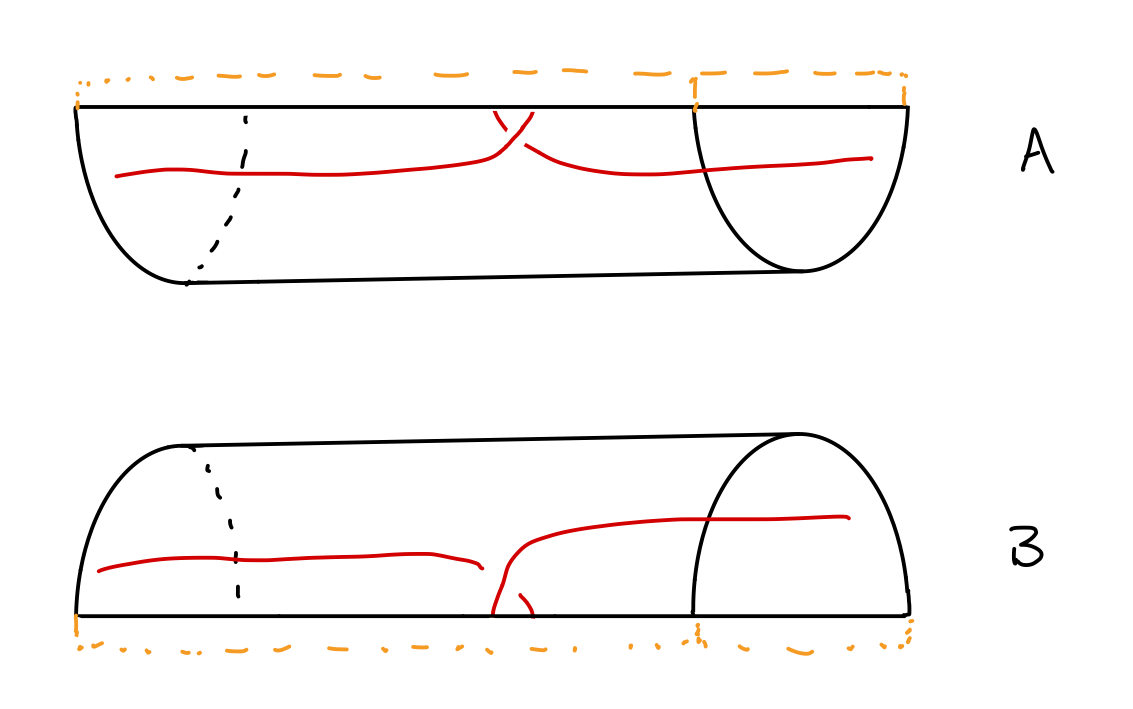
\includegraphics[scale=.2]{1-1.png} \end{center} 
  so that $X = A \cup B$, and both are open, as the orange section of 
  the diagram represents open neighborhoods taken on the edge of both sections. Note that $A \cap B$ is nonempty. 
  Clearly, $A \cong B$, and both can be deformation retracted into spheres with two arcs inside: 
  \par \begin{center} 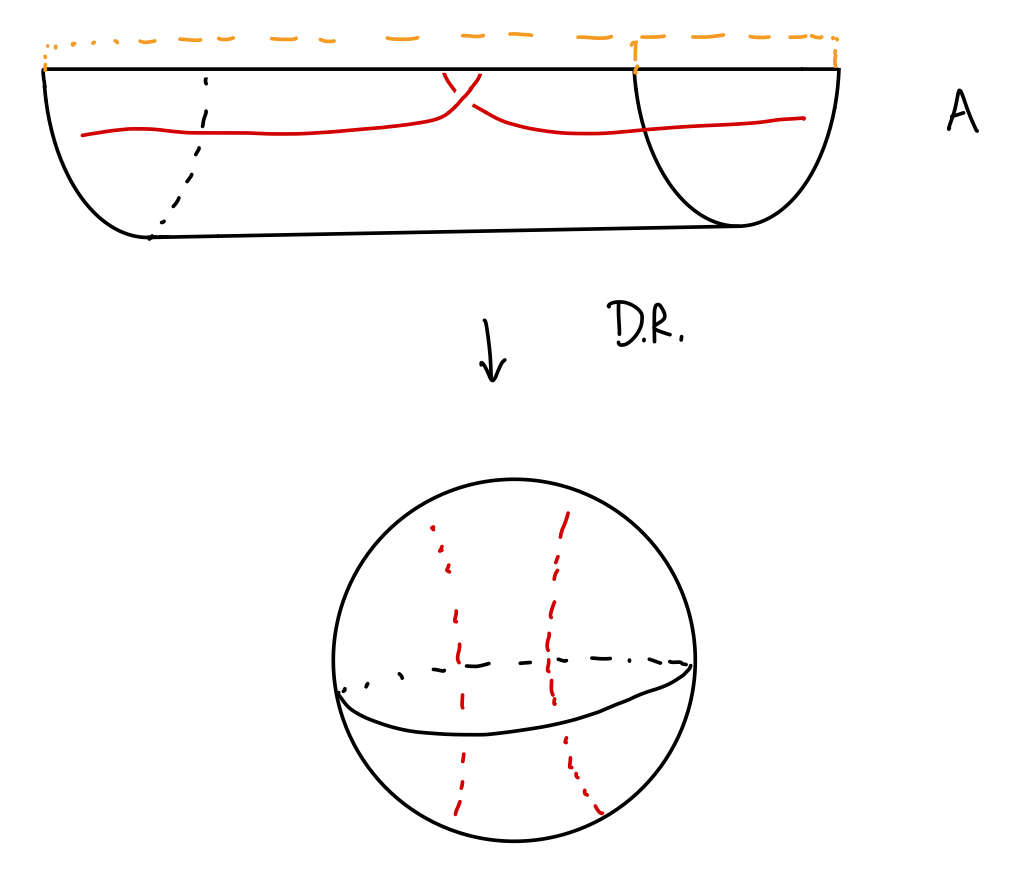
\includegraphics[scale=.2]{1-2.png} \end{center}
  From here, we can find that this actually ends up being homotopically equivalent to two tori wedged summed. 
  \par \begin{center} 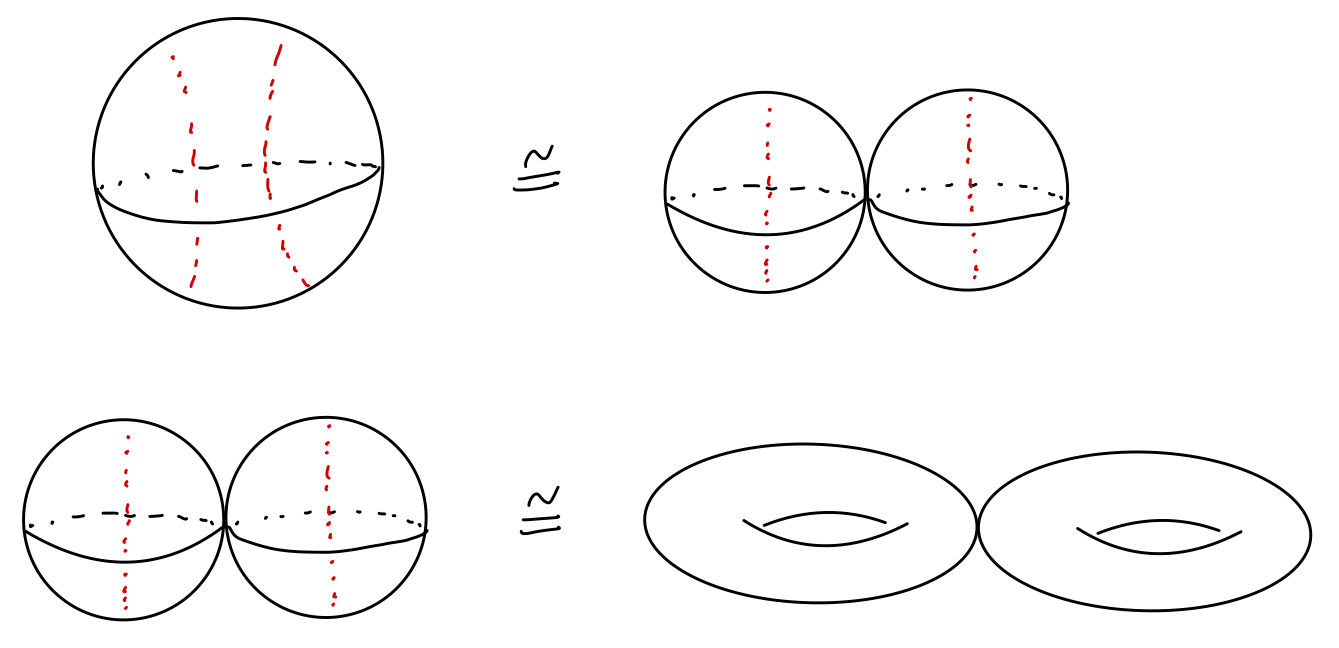
\includegraphics[scale=.2]{1-3.png} \end{center} 
  So the fundamental group for both $A$ and $B$ is $\pi_1(S^1 \times D^2) = \mathbb{Z} * \mathbb{Z}$. Choose a 
  basepoint in the middle of $\alpha$ and $\beta$. 
  \par \begin{center} 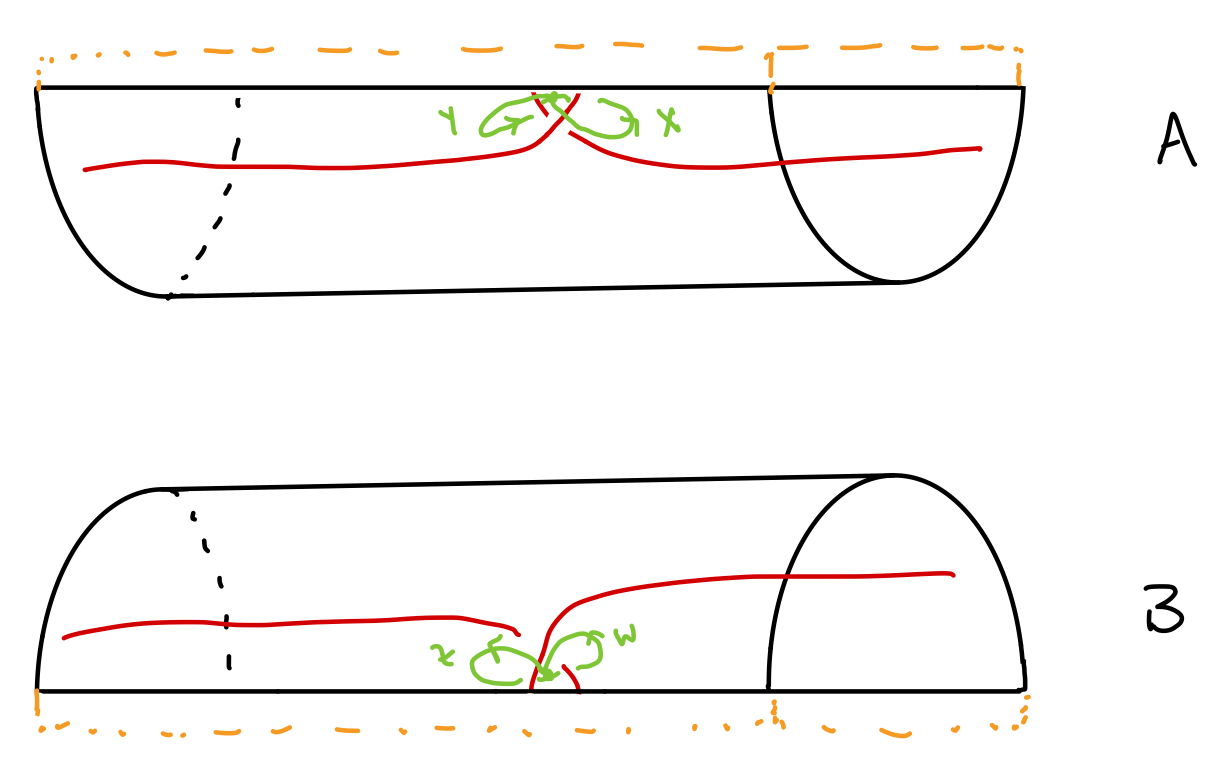
\includegraphics[scale=.2]{1-4.png} \end{center}
  Then, we see that the intersection of $A$ and $B$ deformation retracts to a rectangle missing 2 points, so $\pi_1(A \cap B) = \mathbb{Z} * \mathbb{Z}$. 
  \par \begin{center} 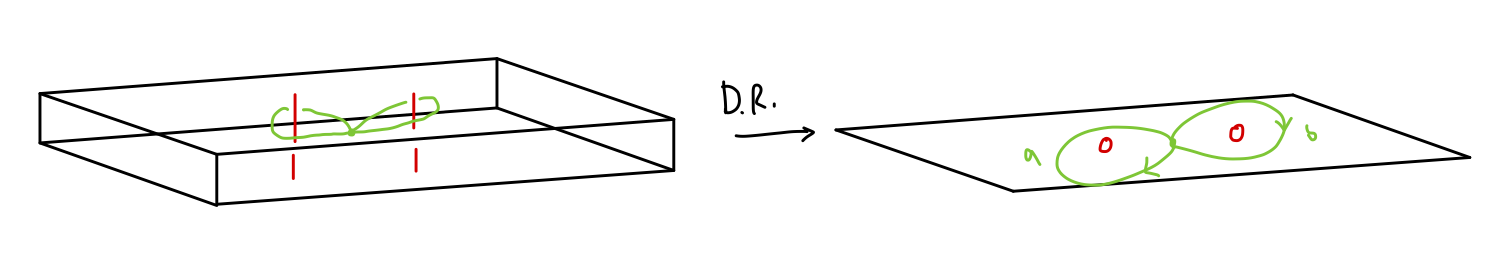
\includegraphics[scale=.2]{1-5.png} \end{center}
  Then we can use Van Kampen:
  \par \begin{center} 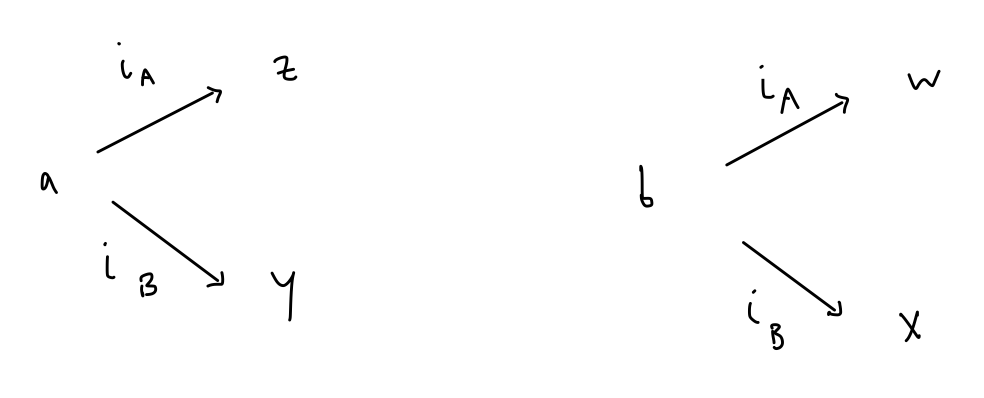
\includegraphics[scale=.2]{1-6.png} \end{center}
  From here we see that 
  \begin{equation*}
    \pi_1(X) = \langle x,y,z,w \vert z=y,w=x \rangle = \langle x,y \rangle = \mathbb{Z} * \mathbb{Z} 
  \end{equation*}
  Next, let's decompose $\gamma$ in the following manner: 
  \par \begin{center} 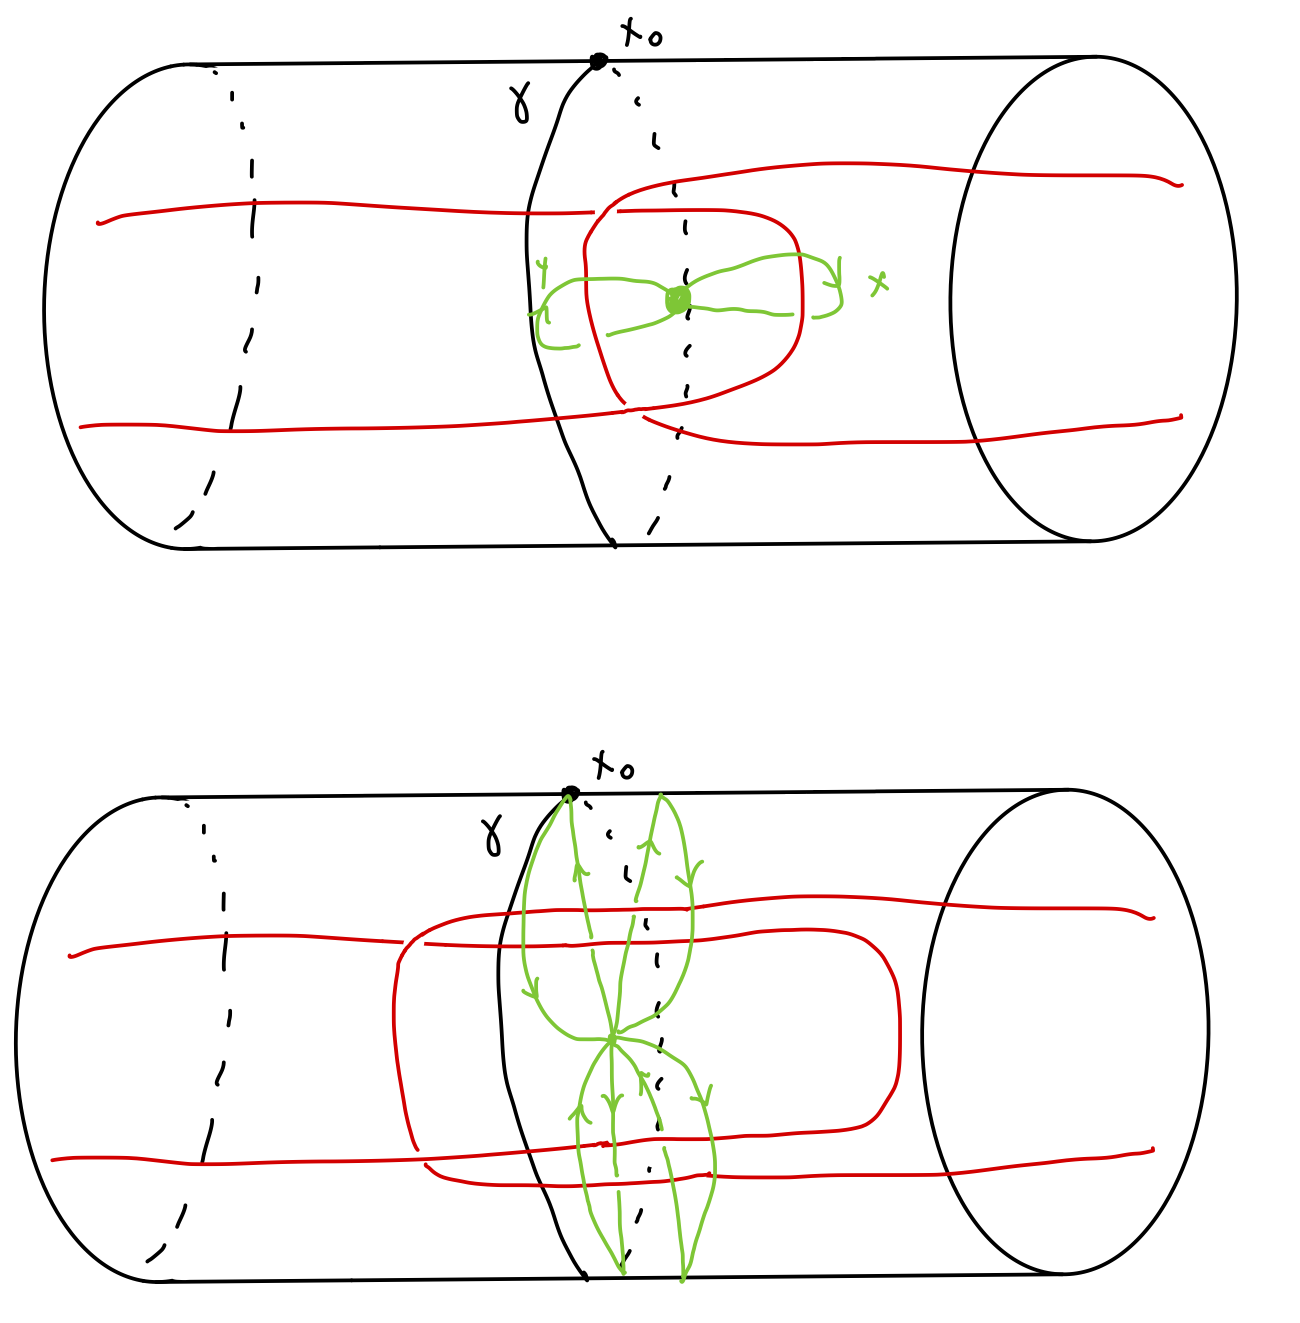
\includegraphics[scale=.2]{1-7.png} \end{center}
  so that it goes around the arcs one at a time. Here, it is clear to see that $[ \gamma ] = [xyx^{-1}y^{-1}]$, 
  which is not the identity in $\langle x,y \rangle$. Thus $\gamma$ cannot be nullhomotopic.
\end{proof}

\begin{statement}[Problem]{2}
  Consider the quotient space of a cube $I^3$ obtained by identifying each square face with the opposite
  square face via the right-handed screw motion consisting of a translation by one unit in the direction 
  perpindicular to the face combined with a one-quarter tqist of the face about it's center point. Show 
  this quoitent space $X$ is a cell complex with two 0-cells, four 1-cells, three 2-cells, and one 3-cell. 
  Using this structure, show that $\pi_1(X)$ is the quaternion group $\{ \pm 1, \pm i, \pm j, \pm k \}$, 
  of order eight. 
\end{statement}
\begin{proof}
  When identifying the sides as described, one pair at a time, the following changes occur to the cube:
  \par \begin{center} 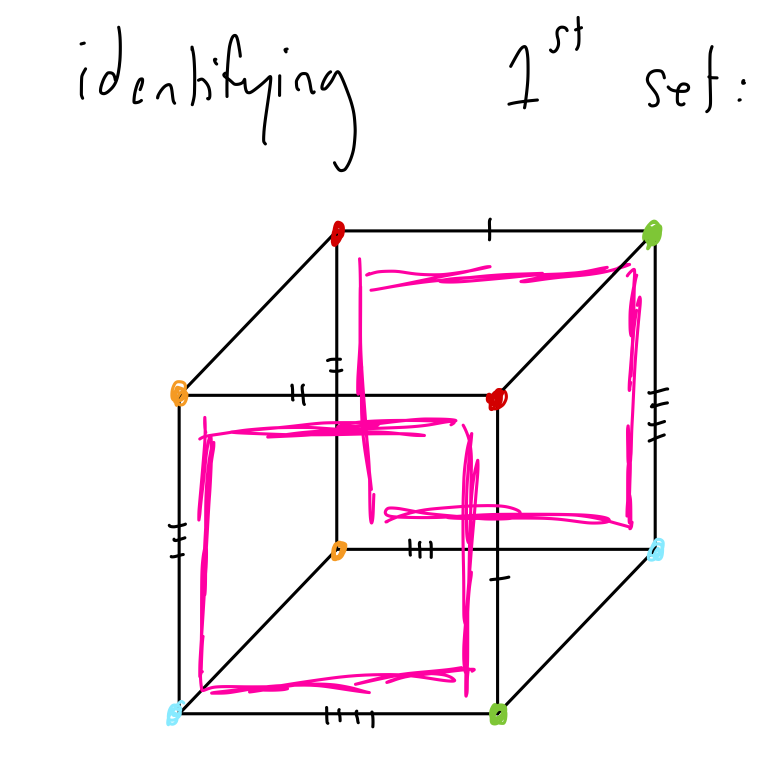
\includegraphics[scale=.2]{2-1.png} \end{center} 
  \par \begin{center} 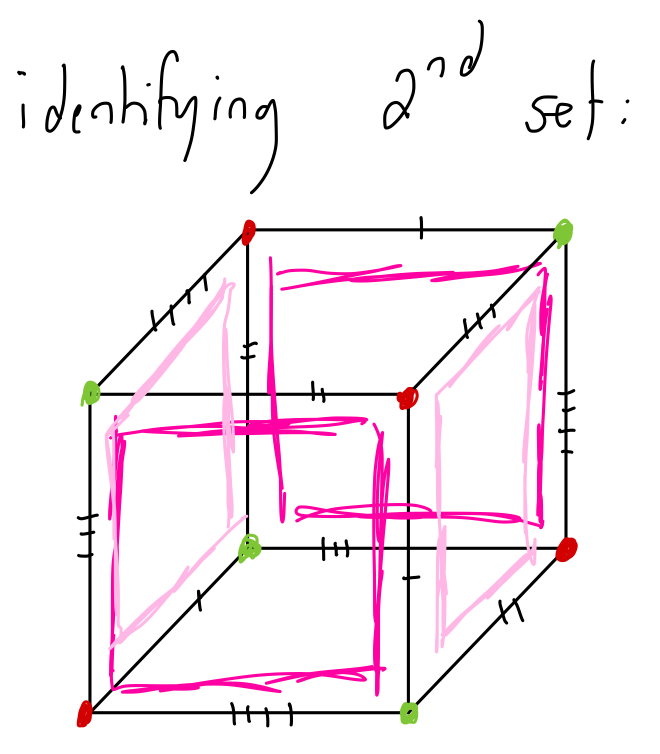
\includegraphics[scale=.2]{2-2.png} \end{center} 
  \par \begin{center} 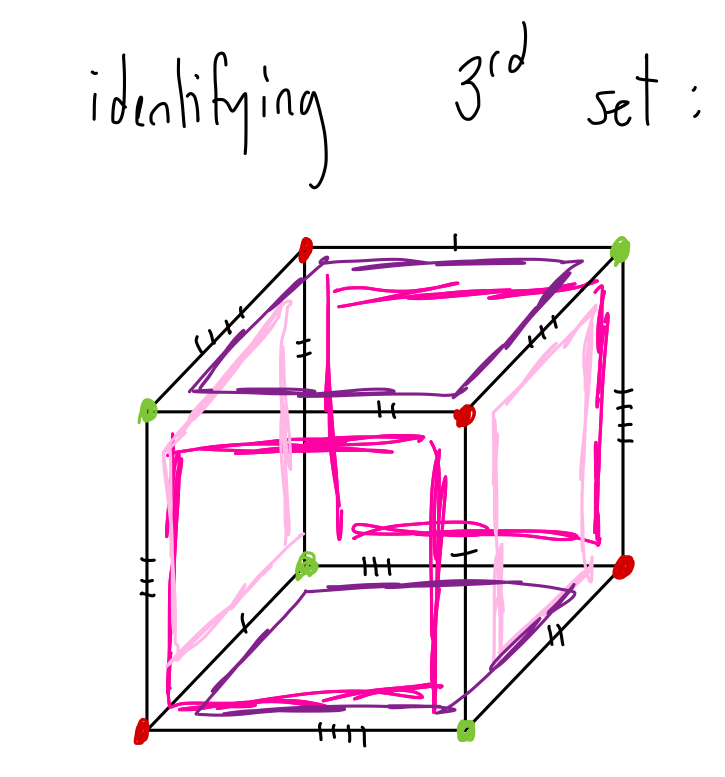
\includegraphics[scale=.2]{2-3.png} \end{center} 
  \par Clearly, we are left with two 0-cells, four 1-cells, three 2-cells, and one 3-cell. If we let the side labeled III be $a$, 
    II be $b$, I be $c$, and IIII be $d$, we get the following representation:
    \begin{equation*}
      \pi_1(X) = \frac{ \langle ab^{-1}, ac^{-1}, ad^{-1} \rangle }{ \langle bc^{-1}ad^{-1}, ba^{-1}dc^{-1}, ac^{-1}db^{-1} \rangle}.
    \end{equation*}
    Then we can let $i=ab^{-1}$, $j=ac^{-1}$, and $k=ad^{-1}$, so that we get 
    \begin{equation*} 
      \pi_1(X) = \frac{ \langle i,j,k \rangle }{ \langle i^{-1}jk, i^{-1}k^{-1}j, jk^{-1}i \rangle}.
    \end{equation*}
    Which is equivalent to 
    \begin{equation*}
      \pi_1(X) = \langle i,j,k \vert i^2 = k^2 = j^2 = ijk \rangle 
    \end{equation*}
\end{proof}

\begin{statement}[Problem]{3}
  Construct a simply-connected covering space of the space $X \subset \mathbb{R}^3$ that is the union 
  of a sphere and a diameter. Do the same when $X$ is the union of a sphere and a circle intersecting
  at two points. 
\end{statement}
\begin{proof}
  \par For the first case, where $X$ is a sphere with a diameter, to make a simply-connected cover we have to find a 
  way for loops to "go around" the diameter in the center of the sphere. To accomplish this, we can make the cover
  infinite spheres, all centered in the center of the sphere, of increasing sizes up until the boundary of the original
  sphere in $X$. Thus if a loop is made, it can be shrunk down the sphere's infinitely and contract to a point, 
  avoiding the diameter. Clearly, this is equivalent to saying the open cover is simply-connected.
  A diagram to better illustrate this: 
  \par \begin{center} 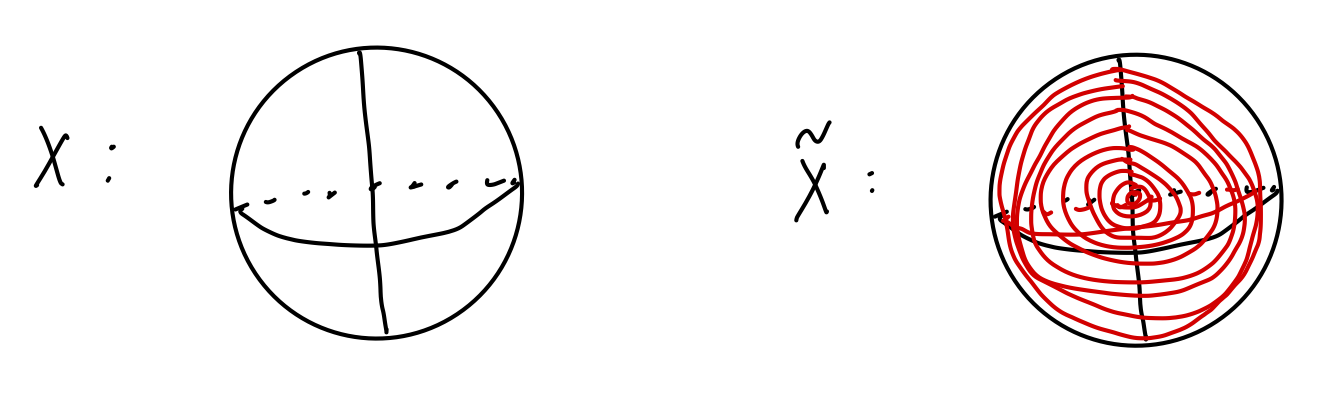
\includegraphics[scale=.2]{3-1.png} \end{center} 
  \par For the second case, where $X$ is a sphere with an $S^1$ intersecting at two points, we have to let loops 
  "get around" the portion of the sphere that is cut off by the intersection. First note that a general cover 
  for $S^1$ is $\mathbb{R}$. Using this fact, we can construct the cover to be infintely many copies of the sphere from 
  $X$ along $\mathbb{R}$, so that no matter where a starting point is on $S^1$, it will always be infinitely
  close to a sphere, where the loop can be contracted to a point.
\end{proof}

\begin{statement}[Problem]{4}
  Let $Y$ be the \textit{quasi-circle} shown in the figure, a closed subspace of $\mathbb{R}^2$ 
  consisting of a portion of the graph of $y = \sin(\frac{1}{x})$, the segment $[-1,1]$ in 
  the $y$-axis, and an arc connecting these two peices. Collapsting the segment of $Y$ in the $y$-axis 
  to a point gives a quoitent map $f: Y \to S^1$. Show that $f$ does not lift to the covering space 
  $\mathbb{R} \to S^1$, even though $\pi_1(Y)=0$. Thus local path-connectedness of $Y$ is a 
  necessary hypothesis in the lifting criterion. 
\end{statement}
\begin{proof}
  First, assume that $f([-1,1])=\{1\}$, and let $\tilde{f}:Y \to \mathbb{R}$ be a lift. Because $Y \setminus [-1,1]$ 
  is connected, $\tilde{f}(Y \setminus [-1,1])$ must also be connected. Because it is connected, 
  it must lay on some component of $p^{-1}(f(Y \setminus [-1,1])) = \mathbb{R} \setminus 2\pi \mathbb{Z}$.
  Because $f$ is surjective, that $\tilde{f}(Y \setminus [-1,1])$ must be $(0, 2\pi)$. 
  From here, by the fact that $Y$ is compact, we know $[0,2\pi] \subset \tilde{f}(Y)$. Thus 
  $\{0,2\pi \} \subset \tilde{f}([-1,1])$, but clearly $\tilde{f}([-1,1])$ must be a singular point. 
  Therefore we have a contradiction, and $f$ cannot lift to the covering space.
\end{proof}

\begin{statement}[Problem]{5}
  Show that if a path-connected, locally path-connected space $X$ has $\pi_1(X)$ finite, then 
  every map $X \to S^1$ is nullhomotopic. 
\end{statement}
\begin{proof}
  Let $f: X \to S^1$, with $p: \mathbb{R} \to S^1$ the covering map. $f_*(\pi_1(X)) \subset \pi_1(S^1)$, but 
  $f_*(\pi_1(X))$ is finite, and so it must be trivial. Then $f_*(\pi_1(X)) \subset p_*(\pi_1(\mathbb{R}))$.
  By the Lifting Criterion, there exists a lift $\tilde{f}:X \to \mathbb{R}$. Define 
  $f_t: X \times I \mathbb{R}$ be the straight line homotopy between $\tilde{F}$ to a constant map. 
  Then $p \circ f_t$ being a homotopy from $f$ to a constant map proves $f$ is nullhomotopic.
\end{proof}

\begin{statement}[Problem]{6}

\end{statement}
\begin{proof}
  Running out of time, but I know the number of sheets in a covering space is the amount of times a point is 
  covered by the cover. 
\end{proof}

\begin{statement}[Problem]{7}

\end{statement}
\begin{proof}
  Still running out of time, so all I'll say is that $\pi_1(S^1 \vee S^1) = \mathbb{Z} * \mathbb{Z}$.
\end{proof}

\begin{statement}[Problem]{8}

\end{statement}
\begin{proof}
  Running out of time! But I don't want to leave this blank, so I'll say $\mathbb{R}P^2$ is just $\mathbb{R}^2$ minus the origin, and 
  can be thought about as $S^2 \setminus \sim$ where $x \sim -x$.
\end{proof}

\end{document}
